\section{Systemarchitektur}

\subsection{Komponentenübersicht}

\begin{figure}[H]
	\centering
	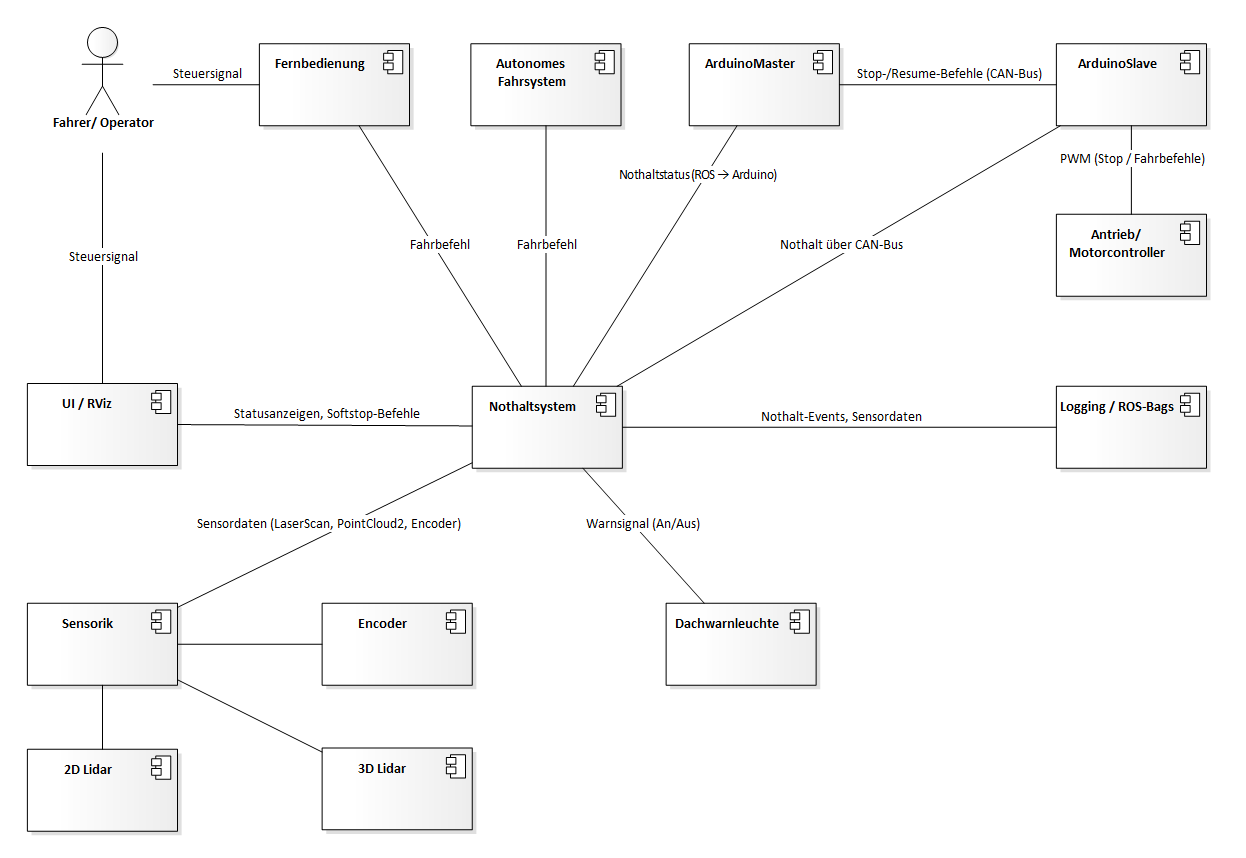
\includegraphics[width = \imglarge]{images/Systemkontext_Nothaltsystem.png}
	\caption{Komponentenübersicht des Nothaltesystems}
	\label{fig:komponentenuebersicht}
\end{figure}

\quad Die Architektur des Nothaltesystems basiert auf einer klar strukturierten Aufteilung in Sensorik, zentrale Entscheidungslogik, Bedienkomponenten, Kommunikationsknoten sowie Aktorik. Das Klassendiagramm veranschaulicht die wesentlichen Systemkomponenten und ihre Beziehungen.

\begin{itemize}
    \item \textbf{SensorSystem}\\
    Liefert die Distanzdaten der 2D- und 3D-LiDAR-Sensorik. Diese Informationen werden von der zentralen NothaltNode ausgewertet.

    \item \textbf{OperatorUI}\\
    Ermöglicht dem Operator das Auslösen von Softstop- und Resume-Befehlen über Taster oder grafische Benutzeroberfläche.

    \item \textbf{NothaltNode}\\
    Zentrale Komponente des Systems. Sie verarbeitet Sensorwerte, bewertet Gefahrenlagen, setzt Zustände (\ac{Hardstop}/\ac{Softstop}/\ac{E-Stop}) und triggert sicherheitsrelevante Aktionen.

    \item \textbf{TruckBridgeNode}\\
    Vermittelt zwischen ROS und dem CAN-basierten Mikrocontrollersystem. Sie überträgt Nothalt- und Freigabekommandos zuverlässig an die Aktorik.

    \item \textbf{MasterArduino}\\
    Empfängt CAN-Kommandos und setzt sicherheitskritische Signale für den SlaveArduino.

    \item \textbf{SlaveArduino}\\
    Wandelt Sicherheitsbefehle in Motor-PWM-Signale um und steuert damit den Motorcontroller.

    \item \textbf{MotorController}\\
    Führt die tatsächliche Bremsung bzw. den Stopp aus.

    \item \textbf{Logger}\\
    Dokumentiert Nothalt-, Sensor- und Zustandsereignisse zur späteren Analyse.
\end{itemize}

\quad Diese Komponenten bilden gemeinsam die technische Basis für einen deterministischen, nachvollziehbaren und sicherheitsorientierten Nothaltprozess.

\subsection{Daten- \& Funktionsflüsse}

\begin{figure}[h]
	\centering
	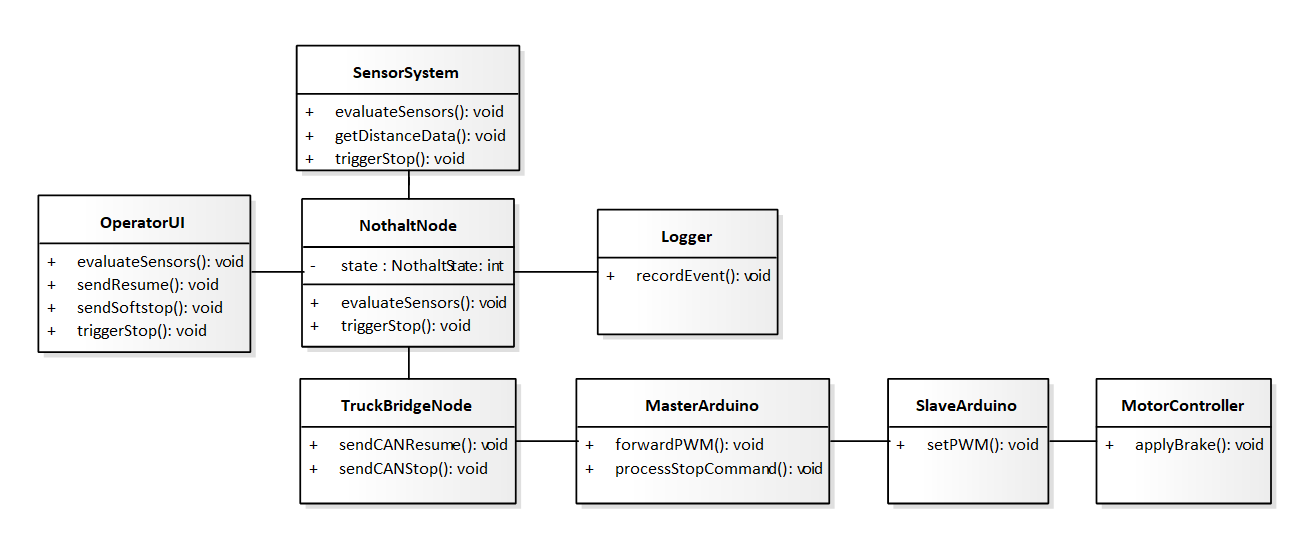
\includegraphics[width = \imglarge]{images/Systemarchitektur.png}
	\caption{Systemarchitektur des Nothaltesystems}
	\label{fig:systemarchitektur}
\end{figure}

\quad Das System folgt einer klaren Datenflusskette vom Erfassen der Umgebung bis zur Umsetzung des Nothalts:

\begin{enumerate}
    \item \textbf{SensorSystem → NothaltNode}\\
    Die NothaltNode erhält kontinuierliche Distanzdaten und bewertet, ob sich Hindernisse in der Warn- oder kritischen Zone befinden.

    \item \textbf{OperatorUI → NothaltNode}\\
    Manuelle Eingaben wie Softstop oder Resume werden direkt an die Entscheidungslogik übergeben.

    \item \textbf{NothaltNode → TruckBridgeNode}\\
    Wird ein Nothalt ausgelöst, sendet die NothaltNode entsprechende Kommandos an die CAN-Bridge.

    \item \textbf{TruckBridgeNode → MasterArduino → SlaveArduino → MotorController}\\
    Der Befehl wird hardwareseitig weitergereicht, bis der Motorcontroller den Stopp ausführt.

    \item \textbf{NothaltNode → Logger}\\
    Alle sicherheitsrelevanten Ereignisse (\ac{Softstop}, \ac{Hardstop}, \ac{E-Stop}, \ac{Resume}) werden aufgezeichnet.
\end{enumerate}

\quad Diese Struktur stellt sicher, dass die Nothaltlogik zentral ausgeführt wird, während die sicherheitskritische Aktorik über dedizierte Hardwarepfade zuverlässig angesprochen wird. Das Zusammenspiel der Klassen gewährleistet ein konsistentes, robustes und erweiterbares Systemdesign.
